% convection, v1.0

\chapter{Convection}~\label{ch:convection}

\paragraph{Abstract} The study of convection in liquid xenon detectors has not at this point been given an exhaustive treatment. While some publications address the topic, no dedicated works on the topic exist. In this chapter we provide some background information about convection in liquid xenon as well as discussion about its measurement.

The analysis of the ${}^{220}$Rn calibration data from XENON100~\cite{Aprile:2016pmc} revealed a buoyancy-driven convection pattern with a considerable $8\1{mm/s}$ fluid speed. A similar analysis from LUX~\cite{Malling:2014} of \Rn~in background data in revealed a pattern with the same features but a higher fluid speed of $3\1{cm/s}$. This was in stark contrast to the lack of convection that was observed in EXO-200~\cite{Albert:2015vma}.

Unless otherwise noted, values for thermodynamic properties of xenon used in this chapter are from NIST~\cite{NIST}.

\section{A review of convection}~\label{sec:convec_review}

The two most common types of convection are natural convection, arising from thermodynamically-driven density gradients, and forced convection, arising from the action of a pump or other device. We will focus here on natural convection, as this dominates over forced convection inside the TPC. The dimensionless quantities commonly associated with natural convection are the Rayleigh and Grashof numbers~\cite{Chandrasekhar:1961,Grashof}, given by

\begin{align}
\n{Ra}_x &= \frac{g\beta\Delta T x^3}{\nu\alpha} = \n{Gr}_x\n{Pr} \\
\n{Gr}_x &= \frac{g\beta\Delta T x^3}{\nu^2}
\label{eq:dimensionless}
\end{align}

Here, $\n{Ra}$ is the Rayleigh number and \n{Gr} the Grashof number, $g$ the earth's gravitational field ($9.8\1{m/s^2}$), $\beta$ the coefficient of thermal expansion ($XX\1{units}$), $\nu$ the kinematic viscosity $XX\1{units}$), $\alpha$ the thermal diffusivity ($XX\1{units}$), $\Delta T$ the temperature difference ($0.3\1{K}$), and $x$ the chracteristic length scale ($1\1{m}$). $\n{Gr}$ relates buoyancy and viscosity, while the Prandtl number $\n{Pr}$~\cite{Prandtl} is the ratio between viscous and thermal diffusion rates and is a function purely of the fluid. For xenon at the temperatures involved here, the value is $XX$.

If we evaluate the Grashof and Rayleigh numbers, we find values of \todo{XX} and \todo{YY} respectively, indicating a laminar boundary layer, and a convection speed of order $\order{XX\1{mm/s}}$.

\section{Convection in XENON1T}~\label{sec:convection}

Given the similarities in the convection patterns between XENON100 and LUX and the differences between how those experiments inject xenon into the active volume, concrete predictions of what to expect in XENON1T are difficult to make. Conceptually, we might expect a similar single-cell pattern, or the increased detector size might allow the formation of two cells. Thus, it is important that any attempt to measure the convection be as agnostic possible, in order to avoid projecting expecations onto the data.

To measure convection we require two decays out of a decay chain so that there is a meaningful correlation between decay vertices. We further impose a number of requirements on these two decays.
\begin{enumerate}
    \item One isotope in the chain must be capable of being injected into the detector and must mix throughout.
    \item The two decays of interest must be easily identifiable and shouldn't confuse position reconstruction in any way.
    \item The livetime of the second decay must be relatively short such that $v_{ave}\tau$ is larger than position reconstruction uncertainties, yet small enough such that within two or three livetimes it's still closer to its parent than any others (to facilitate easy matching).
    \item Any further activity in the decay chain must either decay away quickly or be removable (decay is preferable), unless this measurement is done at the end of the detector's lifetime, in which case this can be relaxed.
\end{enumerate}

Requirememt $(1)$ excludes all decay chains without some gasseous form, or that cannot form some gasseous compount (conceptually similar to $\n{CH}_3\n{T}$ or $\n{UF}_6$). Requirement $(2)$ points towards isotopes that primarily have an $\alpha$ mode, as a high-energy $\gamma$ will scatter multiple times, which makes position reconstruction difficult. Isotopes with $\beta$-decays are difficult to identify due to the lack of defining spectral features. Requirement $(3)$ can be fulfilled by reducing the injected activity, but this then means the measurement requires more time. Furthermore, if the livetime of the second isotope is not short compared to the timescale of convection, this also makes matching difficult, as the effects of curvature of the fluid streamlines will need to be incorporated when the convection map is constructed.

Pairings of radon and polonium are often ideal for this purpose. Both elements tend to decay via $\alpha$ decay and only rarely emit $\gamma$s during the process, which makes clean populations relatively easy to select. Radon, being a noble element, is easy to introduce into the detector and can bypass most purification systems, and, with the exception of \Rn, have no long-lived progeny, fulfilling requirement $(4)$.

\subsection{$^{220}$Rn-$^{216}$Po}

Given how successful the pairing of $^{220}$Rn and $^{216}$Po were for XENON100 for convection measurements, it is a logical place to start for XENON1T. However, as shown in Figure~\ref{fig:rn220}, the only a paucity of the $^{220}$Rn atoms injected into the active volume reach the drift region, with the majority decaying at or below the cathode.

\begin{figure}[htb]
\centering
    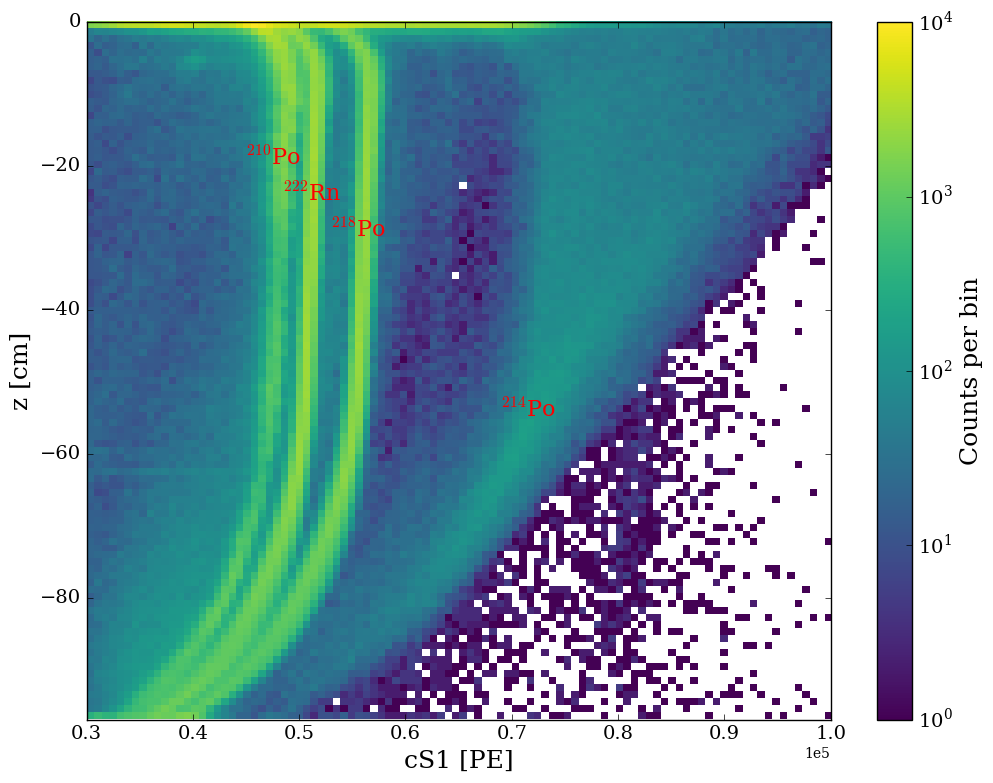
\includegraphics[width=\textwidth]{figures/rnveto/z_cs1}
    \caption{\todo{PLACEHOLDER IMAGE} A plot of {\textit s1\_area\_fraction\_top} (the fraction of the S1 seen by the top PMT array, an excellent proxy for the $z$ coordinate) versus {\textit s1} for the alpha ROI using $^{220}$Rn calibration data. The majority of events are in the very bottom of the detector at or below the cathode, with only a few reaching the drift region where convection can be measured.}\label{fig:rn220}
\end{figure}

\subsection{$^{222}$Rn-$^{218}$Po}

Another available option to match \Po~decays to their parent \Rn~decays. This is a far less trivial endeavour, as the $3.1\1{min}$ half-life of \Po~is quite lengthy, so even at a very modest $1\1{mm/s}$ convection speed, half of all polonium atoms will move 10s of cm away from their parents. Also, the \Rn~background is both boon and bane. As it is mixed uniformly, this provides potential matched pairs in the entire active volume, however no \Rn~or \Po~decays will happen very far from another \Rn~or \Po, which increases the probability of forming incorrect matches.

The \Rn~background rate is $14\1{\mu Bq/kg}$, for a total activity in the active volume of $28\1{mBq}$. The population of \Rn~necessary to provide this activity is easily found via $R = \frac{\dd N}{\dd t} = -\lambda N$, where $R$ is the rate, $\lambda = \ln 2/t_{1/2}$ the decay constant, and $N$ the number of atoms. Thus, we find the \Rn~population size is about $13\,300\1{atoms}$. These will mix uniformly throughout the detector, giving an average distance between \Rn~atoms to be $3.9\1{cm}$. We apply the same calculations for \Po~and find an average population of $7.5\1{atoms}$. The small population of \Po~means the normal Poissonian fluctuations will have a more significant impact than on \Rn.

\subsubsection{Decay identification}

Selection of \Rn~and \Po~is very straightforward. A plot of the reconstructed $z$-coordinate versus cS1 is shown in Figure~\ref{fig:z_cs1} for alpha decays.

\begin{figure}[htb]
\centering
    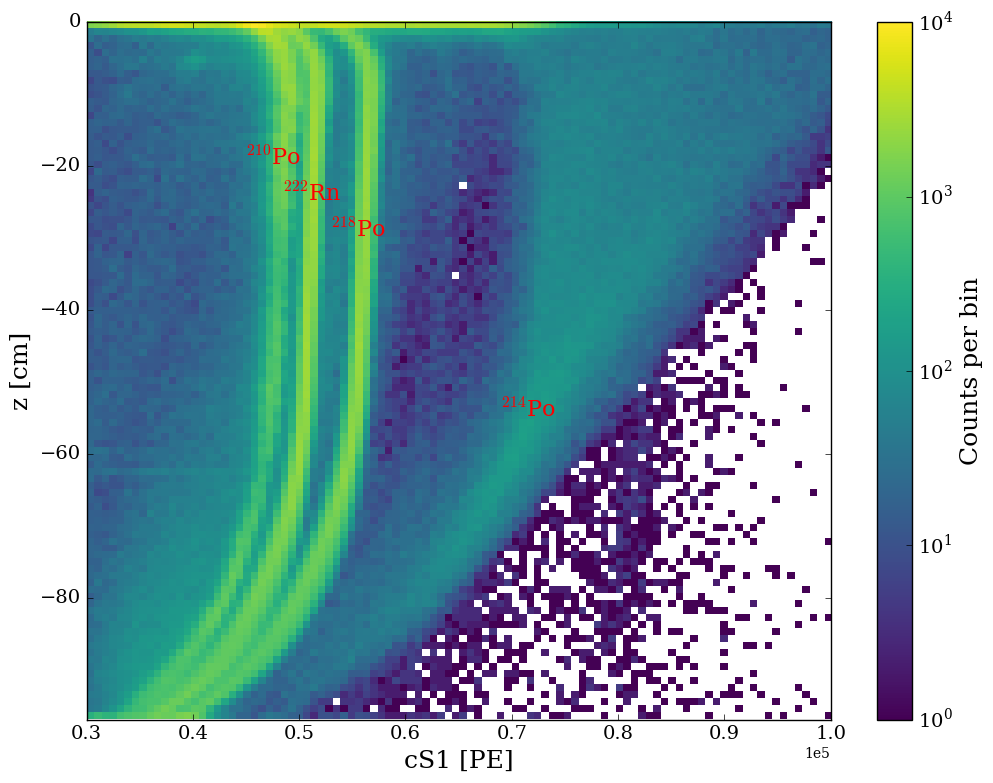
\includegraphics[width=\textwidth]{figures/rnveto/z_cs1}
    \caption{Reconstructed $z$ position versus corrected scintillation light for the alpha ROI. Note the breakdown of the correction factor towards the top and bottom as PMT saturation becomes significant. Four pouplations are evident in the bulk: $^{210}$Po, \Rn, \Po, and $^{214}$Po. The $^{214}$Po is often misreconstructed due to the topology of \BiPo~events deep in the detector, which smears out its population.}\label{fig:z_cs1}
\end{figure}

The $^{210}$Po population exists nearly exclusively on the PTFE reflectors that form the wall of the TPC; a radial cut of even one or two cm significantly reduces its size. The $^{214}$Po band shows up much more clearly if one considers {\it s1\_area\_fraction\_top} rather than $z$, as the short half-life of $^{214}$Po causes some confusion for event reconstruction of the $^{214}$Bi-$^{214}$Po events. The larger S1 from the $^{214}$Po is often paired with the larger S2 from the $^{214}$Bi, resulting in a drift-time that is shorter than the actual value by the livetime of the $^{214}$Po atom.

As we are primarily interested in the center two populations, we can readily select them in the bulk by drawing a few curves on Figure~\ref{fig:z_cs1}, although this tends to break down close to the cathode or liquid surface as the populations smear together. Alternately, machine learning algorithms can exploit separations in multiple parameter spaces simultaneously, providing some additional selection power in these edge regions (see Appendix~\ref{app:ml}).

\subsubsection{Decay matching}

Armed with reasonably clean populations of \Rn~and \Po, the work of decay matching can begin. To do this in as agnostic a fashion as possible, we begin by plotting the temporal and spatial separations of all \Rn~and all \Po~pairs in Figure~\ref{fig:dsdt}. As we can see, most of this parameter space is dominated by random, incorrect pairings. Within a minute after the \Rn~decay, its \Po~daughter merges with the bulk population and cannot be identified with an agnostic approach.

\begin{figure}[htb]
\centering
    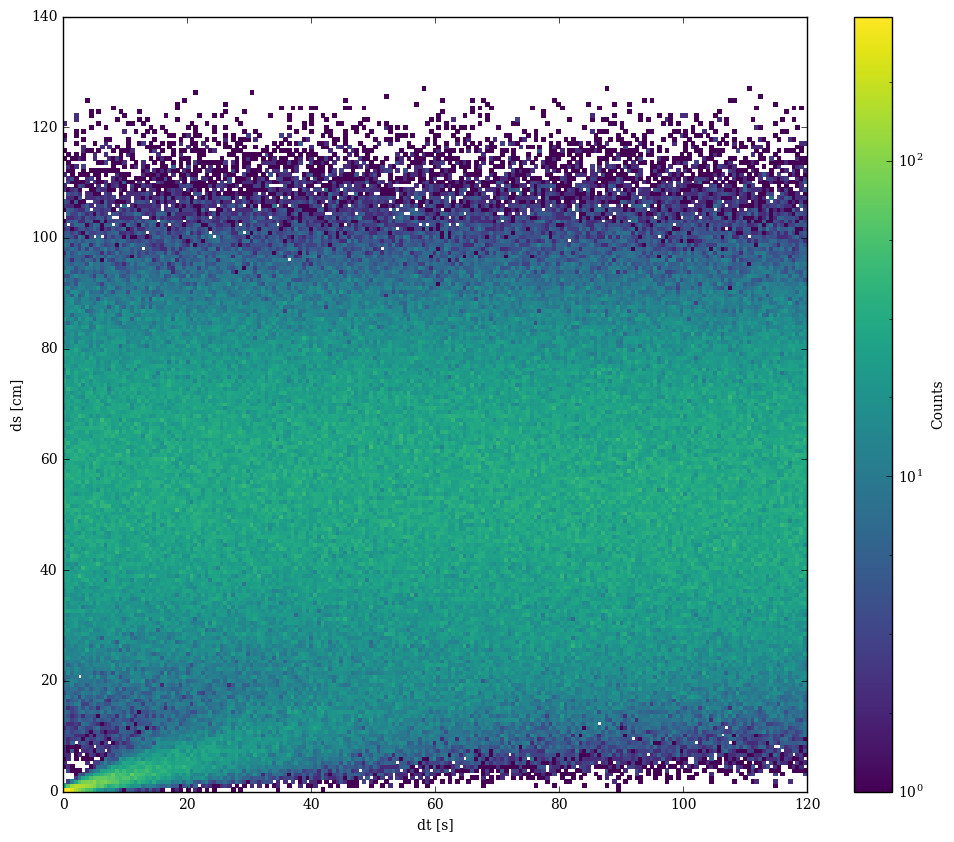
\includegraphics[width=\textwidth]{figures/rnveto/dsdt}
    \caption{Spatial and temporal separations of \Rn~and \Po~events. The ``signal'' population of decay pairs begins at the origin and quickly merges with the ``background'' band of random pairs. Thus, an agnostic approach becomes difficult at times longer than about 45 seconds or distances further than about $15\1{cm}$.}\label{fig:dsdt}
\end{figure}

If we restrict ourselves to potential matches within 30 seconds, this reduces a significant amount of background. Even though this only gives $1-\exp \lambda_{\mathrm{Po}}t = 10\%$ of all possible decays, one day's worth of background data contains some $2500$ total \Rn~decays, or about $7500$ matched decays per month. Evenly spread over the active region, this is one match every $5\1{cm}$, which is sufficient to do a preliminary mapping of convection.

\subsection{Convection map}

By building a three-dimensional map of the displacement of each matched pair we see the shape of the pattern is, as in XENON100 and LUX, a single cell, with much lower speeds of around $3\1{mm/s}$. Figure~\ref{fig:convec} is a projection approximately along the axis of angular momentum.

\begin{figure}[htb]
\centering
    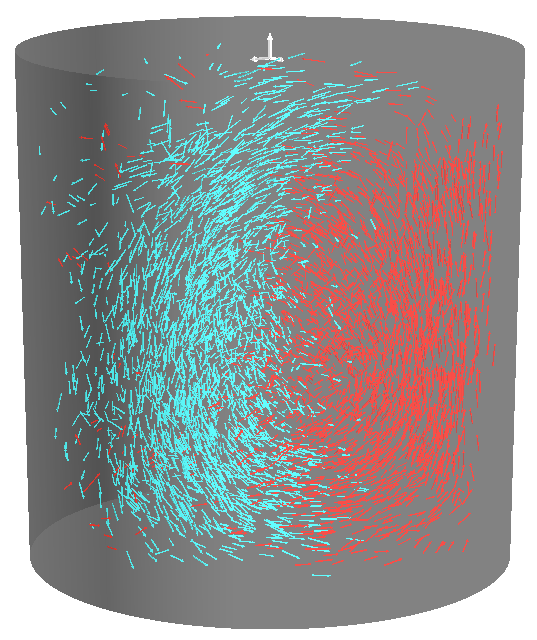
\includegraphics[width=\textwidth]{figures/rnveto/convection_full}
    \caption{The measured convection field in XENON1T. Blue arrows indicates upward movcement; red, downward. A single cell pattern, as was observed in XENON100 and LUX, is clearly seen. Typical speeds are $3\1{mm/s}$.}\label{fig:convec}
\end{figure}

We also see some interesting behavior in the corners. The lack of pairs in these regions indicate a few things. It is unlikely that there is no \Rn~there, but it is entirely possible that our event selection requirements perform very poorly here. This also might be interpreted as hints of counter-current eddies forming in the corners of the detector.

Once a preliminary map is made, this can be used to distinguish correct pairings of \Rn~and \Po~from random matches. The vector connecting two decay verticies should be approximately aligned with the convection cell for correct matches and have a random direction for the incorrect matches. Additionally, because there is at most one \Po~for each \Rn, once a given \Rn~or \Po~has been matched, all other potential matches involving either atom can be removed from consideration.

The combination of these effects allows for an interative process where the matches with the smallest separations (having the best signal to background ratio) are chosen, and any other matches involving these are removed, which reduces the background to all further matches. This can be done again with matches with slightly larger separations.

\section{Simulation}

As the manner of xenon injection in XENON100, LUX, and XENON1T are all different yet all three have the same convection pattern, we can conclude that recirculation does not have a significant impact on convection. Thus, a computational fluid dynamics (CFD) simulation can have some predictive power between experiments, as long as the thermodynamic boundary conditions are correctly modeled. Additionally, a convection field from simulation can probably reveal more about the underlying detector operation than measurements from data.

A variety of different software packages, commercial and otherwise, are available to do this kind of simulation. ANSYS Fluent~\cite{fluent} was used for this work on advice from professor Carlo Scalo of Purdue engineering, also because it is available on the Purdue computing clusters.

A simplified model of the active volume was used to build the simulation mesh, and thermodynamic data from NIST~\cite{NIST} was used at the operating conditions of the detector. The Boussinesq approximation~\cite{Boussinesq:1897} was used to model the density. As we expect laminar, buoyancy-driven flows, the approximation is valid. A representative result is shown in Figure~\ref{fig:cfd_sample}.

\begin{figure}[htb]
\centering
    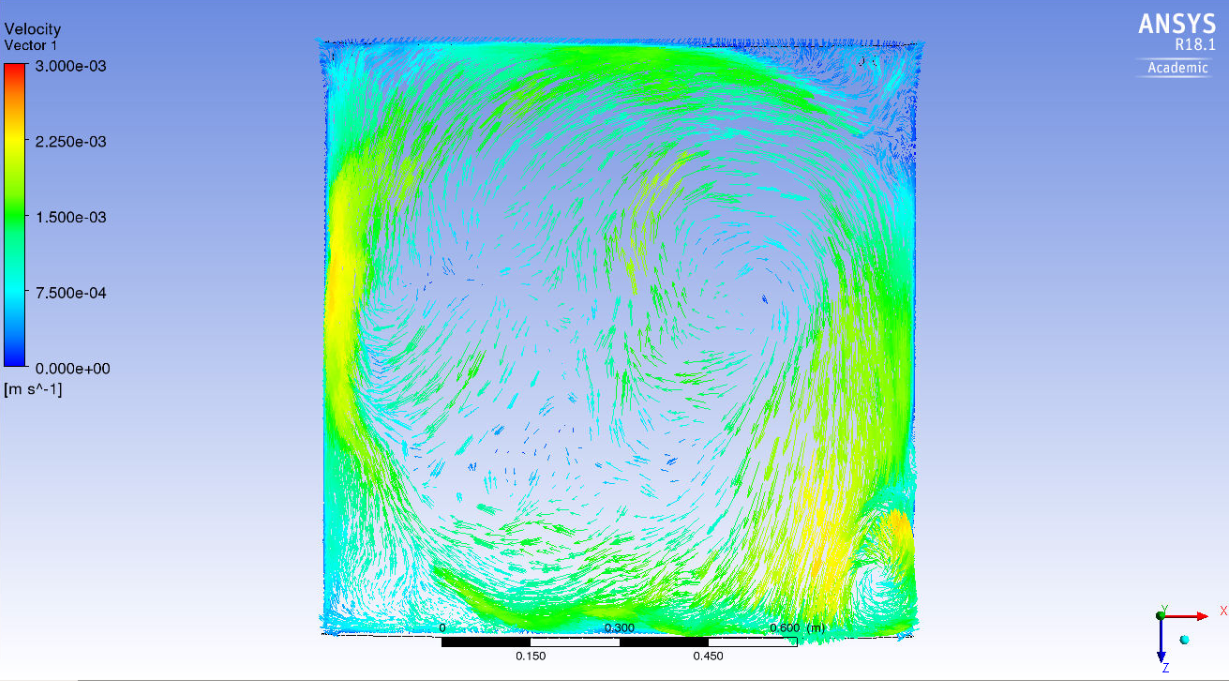
\includegraphics[width=\textwidth]{figures/rnveto/convection_sim}
    \caption{\todo{PLACEHOLDER IMAGE} Simulated convection pattern for XENON1T. A single cell is evident with speeds of a few mm/s. A simple temperature gradient is sufficient to drive this system, though the mechanisms that determine the direction of angular momentum is not yet understood. Counter-currents can be seen in the corners.}\label{fig:cfd_sample}
\end{figure}

Simulations for both steady-state and transient results were performed. The results agree qualitatively with each other, although vortex shedding from counter-currents in the corners are routinely observed.

\section{Comparison between simulation and data}

The simulation results agree qualitatively with the data. A simple temperature gradient is sufficient to establish and drive a single-cell convection pattern, although the symmetry-breaking mechanism that determines the orientation of the pattern is not yet understood. No correlation has been found between the layout of pipes to and from cryogenics and purification and the direction of cell angular momentum.

